
\documentclass[nooutcomes]{ximera}
%\documentclass[space,handout,nooutcomes]{ximera}

% For preamble materials

\usepackage{pgf,tikz}
\usepackage{mathrsfs}
\usetikzlibrary{arrows}
\usepackage{framed}
\usepackage{amsmath}
\pgfplotsset{compat=1.17}

\def\fixnote#1{\begin{framed}{\textcolor{red}{Fix note: #1}}\end{framed}}  % Allows insertion of red notes about needed edits
%\def\fixnote#1{}

\def\detail#1{{\textcolor{blue}{Detail: #1}}}   

\pdfOnly{\renewenvironment{image}[1][]{\begin{center}}{\end{center}}}

\graphicspath{
  {./}
  {chapter1/}
  {chapter2/}
  {chapter4/}
  {proofs/}
  {graphics/}
  {../graphics/}
}

\newenvironment{sectionOutcomes}{}{}


%%% This set of code is all of our user defined commands
\newcommand{\bysame}{\mbox{\rule{3em}{.4pt}}\,}
\newcommand{\N}{\mathbb N}
\newcommand{\C}{\mathbb C}
\newcommand{\W}{\mathbb W}
\newcommand{\Z}{\mathbb Z}
\newcommand{\Q}{\mathbb Q}
\newcommand{\R}{\mathbb R}
\newcommand{\A}{\mathbb A}
\newcommand{\D}{\mathcal D}
\newcommand{\F}{\mathcal F}
\newcommand{\ph}{\varphi}
\newcommand{\ep}{\varepsilon}
\newcommand{\aph}{\alpha}
\newcommand{\QM}{\begin{center}{\huge\textbf{?}}\end{center}}

\renewcommand{\le}{\leqslant}
\renewcommand{\ge}{\geqslant}
\renewcommand{\a}{\wedge}
\renewcommand{\v}{\vee}
\renewcommand{\l}{\ell}
\newcommand{\mat}{\mathsf}
\renewcommand{\vec}{\mathbf}
\renewcommand{\subset}{\subseteq}
\renewcommand{\supset}{\supseteq}
%\renewcommand{\emptyset}{\varnothing}
%\newcommand{\xto}{\xrightarrow}
%\renewcommand{\qedsymbol}{$\blacksquare$}
%\newcommand{\bibname}{References and Further Reading}
%\renewcommand{\bar}{\protect\overline}
%\renewcommand{\hat}{\protect\widehat}
%\renewcommand{\tilde}{\widetilde}
%\newcommand{\tri}{\triangle}
%\newcommand{\minipad}{\vspace{1ex}}
%\newcommand{\leftexp}[2]{{\vphantom{#2}}^{#1}{#2}}

%% More user defined commands
\renewcommand{\epsilon}{\varepsilon}
\renewcommand{\theta}{\vartheta} %% only for kmath
\renewcommand{\l}{\ell}
\renewcommand{\d}{\, d}
\newcommand{\ddx}{\frac{d}{dx}}
\newcommand{\dydx}{\frac{dy}{dx}}


\usepackage{bigstrut}


\title{Trigonometry Checkup}
\author{Bart Snapp and Brad Findell}
\begin{document}
\begin{abstract}
This activity is intended to remind you of key ideas from high school trigonometry. 
\end{abstract}
\maketitle


\begin{problem}
What are the ratios of side lengths in a $45^\circ$-$45^\circ$-$90^\circ$ triangle from shortest to longest, using 1 for the shortest?  $1: \answer{1} : \answer{\sqrt{2}}$. (Hint: Type \texttt{sqrt(2)} for $\sqrt{2}$.)

Explain where the ratios come from, including why they work for any such triangle, no matter what size.  
\begin{hint} Think of half of a square.  Then use the Pythagorean Theorem. \end{hint}
\end{problem}


\begin{problem}
What are the ratios of side lengths in a $30^\circ$-$60^\circ$-$90^\circ$ triangle, from shortest to longest, using 1 for the shortest?  $1 : \answer{\sqrt{3}} : \answer{2}$. 

Explain where the ratios come from.  \begin{hint}Think of half of an equilateral triangle.  Then use the Pythagorean Theorem. \end{hint}
\end{problem}


\begin{problem}
Consider the right triangle below with an angle of $\alpha$, sides of length $x$ and $y$, and hypotenuse of length $r$, as labeled.  
\begin{image}
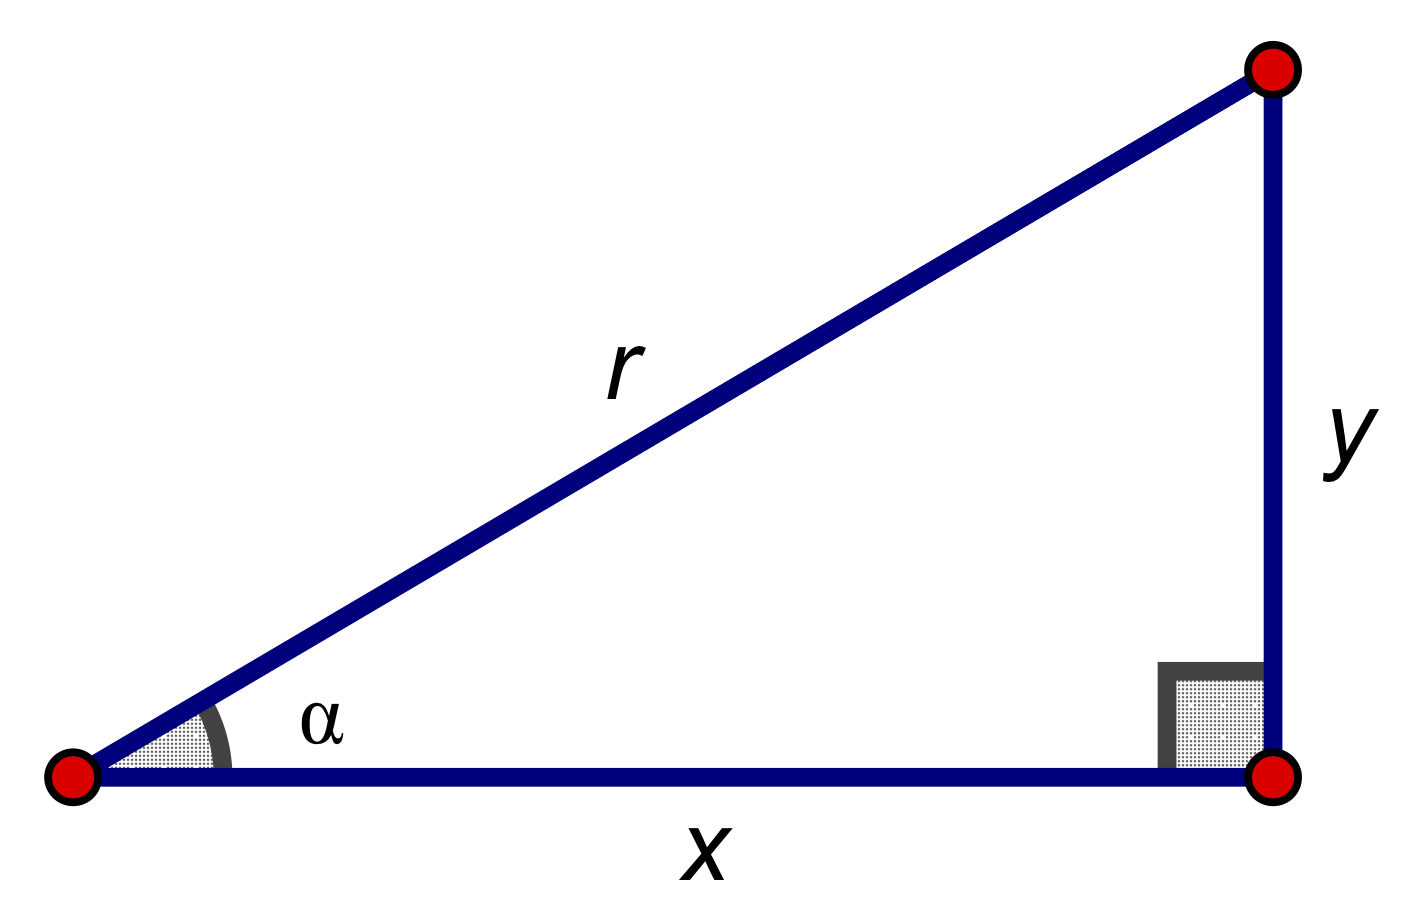
\includegraphics[scale=0.8]{rightTriangle.png}
\end{image}
\begin{enumerate}
\item What values of $\alpha$, measured in degrees, make sense in \emph{right triangle trigonometry}?  (We overcome these bounds for circular trigonometry.)
\[
\answer{0} \le \alpha < \answer{90}
\]  
\item Using the triangle above (and your memory of Precalculus), write down the side-length ratios for sine, cosine, and tangent:  
\[
\sin\alpha = \answer{y/r}, \quad
 \cos\alpha = \answer{x/r}, \quad
  \tan\alpha = \answer{y/x}
\]
\item Now scale the triangle above by $k$, and again write down the side-length ratios for sine, cosine, and tangent:  
\[
\sin\alpha = \answer{y/r}, \quad
 \cos\alpha = \answer{x/r}, \quad
  \tan\alpha = \answer{y/x}
\]
\end{enumerate}
\end{problem}

\begin{problem}
For the problem and triangle above, \dots
\begin{enumerate}
\item If we imagine angle $\alpha$ is fixed, why are ratios of pairs of side lengths the same, no matter the size of the triangle?
  \begin{hint}Because all such right triangles are are similar by AA.  \end{hint}
\item Why is only one of the triangle's three angles necessary in defining these ratios?  
  \begin{hint}The triangle is right, so in fact two angles are known directly.  The third angle can be determined because the sum of the angles is $180^\circ$.\end{hint}  
\item What does it mean to say that these ratios depend upon the angle $\alpha$?  
  \begin{hint}The value of $\alpha$ determines each ratio.  (And a different $\alpha$ gives different ratios.)\end{hint}
\end{enumerate}
\begin{freeResponse}
\end{freeResponse}
\end{problem}

\begin{problem}
Use your work so far to find the following trigonometric ratios:
\begin{enumerate}
\item $\sin 30^\circ = \answer{1/2}, \quad \cos30^\circ = \answer{\sqrt{3}/2}, \quad \tan30^\circ = \answer{1/\sqrt{3}}$.
\item $\sin 45^\circ = \answer{1/\sqrt{2}}, \quad \cos45^\circ = \answer{1/\sqrt{2}}, \quad \tan45^\circ = \answer{1}$.
\item $\sin 60^\circ = \answer{\sqrt{3}/2}, \quad \cos60^\circ = \answer{1/2}, \quad \tan60^\circ = \answer{\sqrt{3}}$.
\item $\sin 0^\circ = \answer{0}, \quad \cos0^\circ = \answer{1}, \quad \tan0^\circ = \answer{0}$.
\end{enumerate}
\end{problem}


\begin{problem}
You may recall the identity $\sin^2\theta+\cos^2\theta=1$.  
\begin{enumerate}
\item Explain why the equation is true.  \begin{hint}For the triangle above, $x^2 + y^2 = r^2$.  Divide both sides by $r^2$, and the equation becomes $\frac{x^2}{r^2} + \frac{x^2}{r^2} = 1$.  From the definitions of sine and cosine and the pictured triangle, it follows that $\sin^2\theta+\cos^2\theta=1$.\end{hint}
\item Why is it called an identity?  \begin{hint}Because the equation is true for all values of the variables.\end{hint}
\item Why is it called a Pythagorean identity?  \begin{hint}Because the proof is essentially a restatement of the Pythagorean Theorem for the pictured triangle.\end{hint}
\end{enumerate}
\begin{freeResponse}
\end{freeResponse}
\end{problem}

\begin{problem}
In right triangle trigonometry, there are two acute angles, as shown in the figure below.
\begin{image}
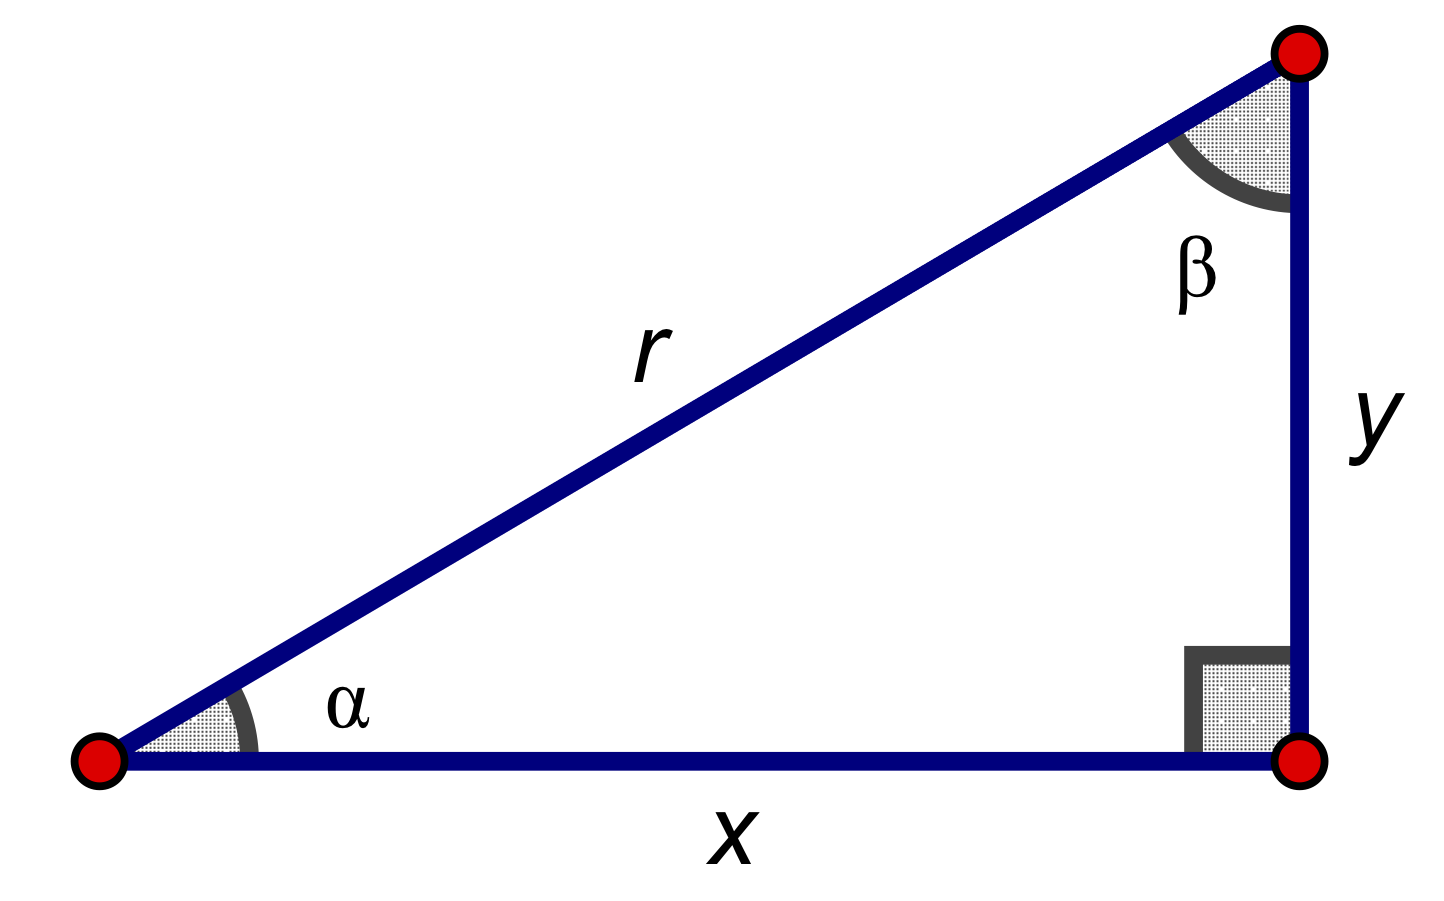
\includegraphics[scale=0.8]{rightTriangle2.png}
\end{image}
\begin{enumerate}
\item How are the angles $\alpha$ and $\beta$ related?  Explain why.  \begin{hint}They are complementary because $\alpha+\beta+90=180$.\end{hint}
\item Using lengths in the above triangle, find the following ratios:    
\[
\sin\alpha = \answer{y/r} \qquad\qquad \cos\alpha = \answer{x/r}
\]
\[
\sin\beta = \answer{x/r} \qquad\qquad \cos\beta = \answer{y/r}
\]
\item We have shown that when angles $\alpha$ and $\beta$ are complementary, 
%\sin\alpha=\answer{\cos\beta} \qquad\textrm{and}\qquad  \cos\alpha = \answer{\sin\beta}
%$\sin\alpha=$\wordChoice{\choice{$\cos\alpha$}\choice{$\sin\beta$}\choice[correct]{$\cos\beta$}} \quad and \quad 
%$\cos\alpha = $\wordChoice{\choice{$\sin\alpha$}\choice[correct]{$\sin\beta$}\choice{$\cos\beta$}}

$\sin\alpha=\answer{\cos\beta}$.  \qquad Enter $\cos\alpha$, $\sin\beta$, or $\cos\beta$.  Type alpha for $\alpha$, beta for $\beta$.  

$\cos\alpha =\answer{\sin\beta}$.  \qquad Enter $\sin\alpha$, $\sin\beta$, or $\cos\beta$.  

\item Explain why the result makes sense.  \begin{hint}We are writing the ratios from the perspective of the other angle, which reverses 
the roles of $x$ and $y$.\end{hint}
\end{enumerate}
\end{problem}

Given an angle and a side length of a right triangle, you can find the missing side lengths.  This is called ``solving the right triangle.''    
And given the sine, cosine, or tangent of an angle, you can find the other two ratios. 

\begin{problem}
Suppose $\sin\alpha = \frac{3}{5}$.  Then $\cos\alpha = \answer{4/5}$, $\tan\alpha = \answer{3/4}$.  
\begin{hint}Draw a right triangle with $\sin\alpha = \frac{3}{5}$, use the Pythagorean Theorem to find the missing side, 
and write down the other trigonometric ratios.\end{hint}
\end{problem}

\begin{problem}
Ethan stands 120 feet from the trunk of a tree (along flat ground). He measures that his line of sight to the top of the tree is at an angle of $53^\circ$ from horizontal. How tall is the tree (above Ethan's line of sight)?  $\answer[tolerance=0.5]{120\tan(53\pi/180)}$

Explain your reasoning.
\begin{hint}Draw a picture with $y$ representing the height of the tree.  From the picture, $\tan 53^\circ = \frac{y}{120}$.  Solve for $y$. \end{hint}
\end{problem}

\begin{problem}
A straight wire to the top of a flagpole meets the ground at a $25^\circ$ angle 30 feet from the base of the flag pole (on a flat lawn).  

How high is the flagpole?  $\answer[tolerance=0.5]{30\tan(25\pi/180)}$

How long is the wire?  $\answer[tolerance=0.5]{30/\cos(25\pi/180)}$
\begin{hint}Draw a picture with $y$ representing the height of the flagpole and $d$ representing the length of wire.  From the picture, $\tan 25^\circ = \frac{y}{30}$.  Solve for $y$.  Also from the picture, $\cos 25^\circ = \frac{30}{d}$.  Solve for $d$. 
\end{hint}
\end{problem}


\end{document}


